\documentclass[a4paper,12pt,oneside]{book}
\usepackage[T1]{fontenc}                                      
\usepackage[utf8]{inputenc}                               
\usepackage[italian]{babel}
\usepackage{amsfonts}
\usepackage{amsthm}
\usepackage{amsmath,amssymb}
\usepackage{array}
\usepackage{arydshln}
\usepackage{braket}
\usepackage{blindtext}
\usepackage{calc}
\usepackage{cancel}
\usepackage{caption}
\usepackage{epsfig}
\usepackage{eucal}
\usepackage{fancyhdr}
\usepackage{geometry}
\usepackage{graphicx}
\usepackage{indentfirst}
\usepackage{hhline}
\usepackage{hyperref}
\hypersetup{
			colorlinks=true,
			linkcolor=black,
			anchorcolor=black,
			citecolor=black,
			urlcolor=black,
			pdftitle={Appunti di Meccanica Quantistica},
			pdfauthor={Vittorio Lubicz}
}

\usepackage{latexsym}
\usepackage{listings} 
\usepackage{longtable}
\usepackage{makeidx}
\usepackage{mathrsfs}
\usepackage{mathdots}
\usepackage{multirow}
\usepackage{nicefrac}
\usepackage{pdfpages}
\usepackage{physics}
\usepackage{setspace}
\usepackage{tikz}
\usepackage{tikz-3dplot}
\usepackage{textcomp}
\usepackage{titlesec,color}
\usepackage{vmargin}
\setpapersize{A4}
\setmarginsrb{35mm}{30mm}{35mm}{30mm}%
             {0mm}{10mm}{0mm}{10mm}



\definecolor{gray75}{gray}{0.75}
\newcommand{\hsp}{\hspace{20pt}}

\titleformat{\chapter}[hang]{\huge\bfseries}{\myfont{\textit{\large{\chaptername\hspace{1pt} \thechapter\hspace{3pt}}}}\textcolor{gray75}{$\mid$}\hspace{0.4cm}}{0pt}{\myfont{\huge\bfseries}}

\titleformat{\section}[hang]{\large\bfseries}{\myfont{\textit{\normalsize{\thesection\hspace{2pt}}}}\hspace{0.4cm}}{0pt}{\myfont{\Huge\bfseries}}

\titleformat{\subsection}[hang]{\large\bfseries}{\myfont{\textit{\small{\thesubsection\hspace{2pt}}}}\hspace{0.4cm}}{0pt}{\myfont{\huge\bfseries}}

\renewcommand{\chaptermark}[1]{\markboth{#1}{}}
\renewcommand{\sectionmark}[1]{\markright{#1}}
\newcommand*{\myfont}{\fontfamily{ppl}\selectfont}

\begin{document}

%*****************LAYOUT PAGINE**************************
\fancypagestyle{plain}{%
\fancyhf{} % cancella tutti i campi di  intestazione e pi\`e di pagina
\fancyfoot[C]{\bfseries \myfont{\thepage}} % tranne il centro
\renewcommand{\headrulewidth}{0pt}
\renewcommand{\footrulewidth}{0pt}}

\fancypagestyle{VS}{
\headheight = 15pt
\lhead[\myfont{\textit{\textbf{\thechapter\nouppercase{\leftmark}}}}]{\myfont{\textit{\textbf{\nouppercase{\leftmark}}}}}
\chead[]{}
\rhead[\myfont{\textbf{\thepage}}]{\myfont{\textbf{\thepage}}}

\lfoot[]{}
\cfoot[]{}
\rfoot[]{}
}
%*******************************************************



\pagestyle{VS}
\setcounter{chapter}{10}
\setcounter{page}{128}
\chapter[Oscillatore Armonico]{Oscillatore Armonico\footnote{S2.3, LL23, G5}}
Consideriamo una particella che compie piccole oscillazioni unidimensionale (il cosidetto \textbf{oscillatore armonico}). L'energia potenziale di tale particella è uguale a $\frac{1}{2}mw^2x^2$, dove $w$ rappresenta nella meccanica classica la frequenza propria delle oscillazioni. L'hamiltoniana dell'oscillatore è quindi:
\begin{equation}
H=\frac{p^2}{2m}+\frac{1}{2}mw^2x^2.
\label{eq:cap11_1}
\end{equation}
Poiché l'energia potenziale diventa infinita per $x=\pm \infty$, la particella può compiere soltanto un moto finito e, di conseguenza,  \textbf{tutto lo spettro} energetico dell'oscillatore \textbf{sarà discreto}.\\
 I livelli energetici dell'oscillatore armonico si possono determinare risolvendo \textbf{l'equazione di Schr\"{o}dinger indipendente dal tempo}:
\begin{equation}
H\psi= -\frac{\hbar^2}{2m}\frac{d^2\psi}{dx^2}+\frac{1}{2}mw^2x^2\psi=E\psi,
\end{equation}
con le condizioni al contorno:
\begin{equation}
\lim _{x \rightarrow \pm \infty} \psi(x)=0.
\end{equation}
Noi invece risolviamo il problema della determinazione dei livelli energetici, e dei relativi autostati, seguendo un elegante \textbf{metodo operatoria sviluppato da Dirac}.
 A tale scopo è conveniente in primo luogo introdurre degli operatori adimensionali, dividendo entrambe i membri dell'equazione (\ref{eq:cap11_1}) per $\hbar w$:
\begin{equation} \label{eq:cap11_2}
\frac{H}{\hbar w}=\frac{p^2}{2m\hbar w}+\frac{mw^2x^2}{2\hbar w}.
\end{equation}
Definendo allora:
\begin{eqnarray}  
	& &\hat{H}=\frac{H}{\hbar w},  \\
	& &\hat{p}=\frac{p}{\sqrt{\hbar w m}},  \\
	& &\hat{x}= \sqrt{\frac{mw}{\hbar}}x,
\end{eqnarray}
possiamo scrivere la precedente equazione nella forma:
\begin{equation}
\hat{H}=\frac{1}{2} (\hat{p}^2+\hat{x}^2).
\end{equation}
Calcoliamo il commutatore tra $\hat{p}$ e $\hat{x}$:
\begin{equation}
[\hat{p},\hat{x}]= \frac{1}{\sqrt{\hbar w m}} \sqrt{\frac{mw}{\hbar}} [p,x]=\frac{1}{\hbar}(-i\hbar),
\end{equation}
ossia:
\begin{equation}  \label{eq:cap11_3}
[\hat{p},\hat{x}]=-i.
\end{equation}
In termini degli operatori $\hat{p}$ ed $\hat{x}$ risulta poi conveniente definire due operatori non hermitiani:
\begin{equation} \label{eq:cap11_4}
\begin{split} 
	a=\frac{1}{\sqrt{2} } (\hat{x}+i\hat{p}), \\
	a^+=\frac{1}{\sqrt{2} } (\hat{x}-i\hat{p}),
\end{split} \end{equation}
o, più semplicemente:
\begin{equation} 
\begin{split}
	a=\sqrt{\frac{mw}{2\hbar}}(x+i \frac{p}{mw}), \\
	a^+=\sqrt{\frac{mw}{2\hbar}}(x-i \frac{p}{mw}).
\end{split}
\end{equation}
Facendo uso della regola di commutazione canonica (\ref{eq:cap11_3}) possiamo calcolare il commutatore tra $a$ e $a^+$:
\begin{equation}
[a,a^+]=\frac{1}{2} [\hat{x}+i\hat{p},\hat{x}-i\hat{p}]=\frac{1}{2}  \left( +i[\hat{p},\hat{x}]-i[\hat{x},\hat{p}]   \right ) = i[\hat{p},\hat{x}],
\end{equation}
e dunque:
\begin{equation}
\mathbf{[a,a^+]=1}.
\end{equation}
Esprimiamo l'operatore $\hat{H}$ in termini degli operatori $a$ e $a^+$. A tale scopo invertiamo le equazioni (\ref{eq:cap11_4}) per ottenere:
\begin{equation} \label{eq:cap11_5}
\begin{split} 
	\hat{x}=\frac{1}{\sqrt{2} } (a+a^+), \\
	\hat{p}=\frac{1}{\sqrt{2}i } (a-a^+).
\end{split}
\end{equation}
Si trova allora:
\begin{eqnarray}
	\hat{H} &=& \frac{1}{2} (\hat{p}^2+\hat{x}^2)=  \frac{1}{4} \left[ -(a-a^+)^2+(a+a^+)^2  \right]= \nonumber\\
	&= &\frac{1}{4} (aa^++a^+a)\cdot 2= \frac{1}{2}(aa^++a^+a)= \nonumber\\
	&=&\frac{1}{2}( [a,a^+]+2a^+a  )=\frac{1}{2}(1+2a^+a ),
\end{eqnarray}
ossia:
\begin{equation} 
\begin{split}
	\hat{H} =a^+a +\frac{1}{2}.
\end{split}
\end{equation}
Equivalentemente:
\begin{equation} \label{eq:cap11_6}
\begin{split}
	H =(a^+a+ \frac{1}{2}) \hbar w.
\end{split}
\end{equation}
Per comprendere il significato degli operatori $a$ e $a^+$ supponiamo di conoscere un autovalore $E_n$  dell'energia ed il corrispondente autostato $|n \rangle$:
\begin{equation}
H|n\rangle=E_n|n\rangle.
\end{equation}
Consideriamo quindi l'applicazione di H allo stato ottenuto applicando l'operatore $a$ ad $|n\rangle$:
\begin{equation}
Ha|n\rangle= [H,a]|n \rangle+aH|n\rangle=([H,a]+E_na)|n\rangle.
\end{equation}
Calcoliamo il commutatore [H,$a$]:
\begin{eqnarray}
	[H,a]&=&\hbar w[a^+a+\frac{1}{2},a]=\hbar w [a^+a,a]= \nonumber\\
	&=&\hbar w (a^+aa-aa^+a)=\hbar w[a^+,a]a=-\hbar wa.
\end{eqnarray}
Allora:
\begin{equation}
Ha|n\rangle=(E_n-\hbar w)a|n\rangle.
\end{equation}
Pertanto, se \textbf{$\mathbf{|n\rangle}$ è un autostato dell'hamiltoniana con autovalore $E_n$ allora anche $a|n\rangle$ è  un autostato dell'hamiltoniana con autosalone $E_n$-$\hbar w$. Per questa ragione l'operatore $a$ è anche detto \textit{operatore di distruzione}}.  \\
 Similmente possiamo considerare l'applicazione di H sullo stato $a^+|n\rangle$:
\begin{equation}
Ha^+|n\rangle= [H,a^+]|n\rangle+a^+H|n\rangle=([H,a^+]+E_na^+)|n\rangle.
\end{equation}
Il commutatore di H con $a^+$ risulta:
\begin{eqnarray}
	[H,a^+]&=&\hbar w[a^+a+\frac{1}{2},a^+]=\hbar w [a^+a,a^+]= \nonumber\\
	&=&\hbar w (a^+aa^+-a^+a^+a)=\hbar w a^+ [a,a^+]=\hbar wa^+,
\end{eqnarray}
o anche:
\begin{equation}
[H,a^+]=-[H,a]^+=\hbar w a^+.
\end{equation}
Allora:
\begin{equation}
Ha^+|n\rangle=(E_n+\hbar w)a^+|n\rangle,
\end{equation}
ossia se \textbf{$|n\rangle$ è un autostato dell'hamiltoniana con autovalore $E_n$ allora anche $a^+|n\rangle$ è  un autostato dell'hamiltoniana con autovalore $E_n$-$\hbar w$. Per questa ragione l'operatore $a^+$ è anche detto \textit{operatore di creazione}}. \\ 
 Questi risultati indicano che \textbf{i livelli di energia sono discreti e differiscono tra loro per un numero interno di unità $\hbar w$}.\\
 Un'altra importante osservazione è che gli autovalori dell'energia devono essere sempre positivi, ed anzi, più precisamente, maggiori od uguali di $\hbar w/2$. Si ha infatti:
\begin{eqnarray}
	E_n&=&\langle n|H|n \rangle= \hbar w \langle n|(a^+a+\frac{1}{2})|n\rangle= \nonumber \\
	&=&\hbar w (\langle n|(a^+a)|n\rangle+\frac{1}{2})=\hbar w (\langle n'|n'\rangle+\frac{1}{2}) \geq \frac{1}{2} \hbar w, 
\end{eqnarray}
giacché per qualunque ket $|n'\rangle$ si ha $\langle n'|n' \rangle\geq 0$ (e con $|n'\rangle= a|n\rangle$).
Deve dunque esistere uno \textbf{stato fondamentale}, il cui vettore di stato indicheremo con $|0\rangle$, la cui energia $E_0$ è maggiore o uguale di $\hbar w/2$. Poiché poi l'operatore $a$, se applicato ad un autostato, produce l'autostato di energia inferiore, deve valere la relazione:
\begin{equation}  \label{eq:cap11_7}
\mathbf{a|0\rangle=0}.
\end{equation}
 \textbf{L'energia del livello fondamentale} può essere ora facilmente calcolata:
\begin{equation}
H|0\rangle= \hbar w(a^+a+\frac{1}{2})|0\rangle= \frac{1}{2} \hbar w |0\rangle,
\end{equation}
ossia:
\begin{equation}
E_0=\frac{1}{2} \hbar w
\end{equation}
 I livelli di energia dell'oscillatore armonico risultano dunque dati da:
\begin{equation}
  \label{eq:cap11_8}
E_n=(n+\frac{1}{2}) \hbar w ,
\end{equation}
con   \textbf{n=0,1,2,...}

 L'equazione (\ref{eq:cap11_6}) implica che gli autostati $|n\rangle$ dell'hamiltoniana sono autostati simultanei dell'operatore $a^+a$. L'espressione (\ref{eq:cap11_8}) per gli autovalori dell'energia $E_n$ indica inoltre che i corrispondenti autovalori dell'operatore $a^+a$ sono i numeri interi n. Per tale ragione l'operatore hermitiano $a^+a$ è anche detto \textbf{operatore numero}:
\begin{equation}
\mathbf{N=a^+a},
\end{equation}
e si ha:
\begin{equation}
\mathbf{N|n\rangle=n|n\rangle}.
\end{equation}
\\\\
 Discutiamo ora come gli autostati $|n\rangle$ dell'hailtoniana possono essere costruiti a partire dall'autostato $|0\rangle$ corrispondente allo stato fondamentale dell'oscillatore.
 Il ruolo degli operatori $a$ e $a^+$ come operatori di distruzione e costruzione rispettivamente implica che gli stati $a|n\rangle$ ed $a^+|n\rangle$ coincidono, a meno di una costante di normalizzazione, con gli autostati $|n-1\rangle$ ed $|n+1\rangle$. Possiamo pertanto scrivere:
\begin{equation}
\begin{cases}
a|n\rangle=c_n|n-1\rangle,\\
a^+|n-1\rangle=d_n|n\rangle.
\end{cases}.
\end{equation}
 Per ricavare le costanti $c_n$ e $d_n$ osserviamo innanzitutto che:
\begin{equation}
c_n=\langle n-1|a|n\rangle=\langle n|a^+|n-1\rangle^*=d_n^*.
\end{equation}
 Inoltre, applicando l'operatore numero allo stato $|n\rangle$ troviamo:
\begin{equation}
N|n\rangle=n|n\rangle=a^+a|n\rangle=c_na^+|n-1\rangle=c_nd_n|n\rangle=|c_n|^2|n\rangle,
\end{equation}
ossia:
\begin{equation}
|c_n|^2=n.
\end{equation}
Scegliendo per convenzione $c_n$ reale e positivo (tale scelta essendo sempre possibile giacché i vettori di stato sono definiti a meno di un fattore di fase arbitrario) vediamo allora che $c_n=\sqrt{n}$. In definitiva abbiamo dimostrato le relazioni:
\begin{equation} \label{eq:cap11_9}
\begin{cases}
a|n\rangle= \sqrt{n} |n-1\rangle, \\
a^+|n-1\rangle=\sqrt{n}|n\rangle.
\end{cases}
\end{equation}
Queste relazioni consentono in particolare di costruire tutti gli autostati dell'hamiltoniana applicando in successione l'operatore $a^+$ allo stato fondamentale $|0\rangle$. Otteniamo:\\\\
\begin{eqnarray} \label{eq:cap11_10}  %non so come mandare tutto a sx
& &|1\rangle=a^+|0\rangle \nonumber \\
& &|2\rangle=\frac{1}{\sqrt{2}}a^+|1\rangle=\frac{1}{\sqrt{2}}(a^+)^2|0\rangle \nonumber \\
& &|3\rangle= \frac{1}{\sqrt{3}}a^+|2\rangle=\frac{1}{\sqrt{3!}}(a^+)^3|0\rangle   \\
& &... \nonumber\\
& &|n\rangle=\frac{1}{\sqrt{n!}}(a^+)^n|0\rangle \nonumber
\end{eqnarray}



 Il metodo operatoriale di Dirac consente anche di ricavare le \textbf{f.d.o nello spazio delle coordinate corrispondenti agli autostati dell'energia.}\\
 Consideriamo in primo luogo lo stato fondamentale definito dall'equazione (\ref{eq:cap11_7}). Moltiplicando a sinistra questa equazione per il $\langle x'|$ troviamo:
\begin{equation}
\langle x'|a|0 \rangle= \sqrt{\frac{mw}{2\hbar}}\langle x'|(x+\frac{ip}{mw})|0 \rangle=0.
\end{equation}
Ricordando le espressioni degli operatori x e p nella rappresentazione delle coordinate, otteniamo l'equazione:
\begin{equation} \label{eq:cap11_12}
\sqrt{\frac{mw}{2\hbar}}(x'+\frac{\hbar}{mw}\frac{d}{dx'})\psi_0(x')=0,
\end{equation}
dove si è indicata con:
\begin{equation}
\psi_0(x')=\langle x'|0 \rangle.
\end{equation}
l'autofunzione corrispondente allo stato fondamentale dell'oscillatore. \\
Ponendo:
\begin{equation}
x_0=\sqrt{\frac{\hbar}{mw}} \qquad \textrm{e} \qquad \xi=\frac{x'}{x_0},
\end{equation}
si può riscrivere l'equazione (\ref{eq:cap11_12}) nella forma:
\begin{equation}  \label{eq:cap11_13}
a\psi_o(\xi)=\frac{1}{\sqrt{2}}(\xi+\frac{d}{d\xi})\psi_0(\xi)=0.
\end{equation}
Per inciso vediamo che \textbf{nella rappresentazione delle coordinate, in termini della variabile adimensionale $\xi=x/x_0$, gli operatori di creazione e distruzione si esprimono come}:
\begin{equation}    \label{eq:cap11_14}
\begin{split}
	a=\frac{1}{\sqrt{2}} (\xi+\frac{d}{d\xi}) \\
	a^+=\frac{1}{\sqrt{2}} (\xi-\frac{d}{d\xi}) 
\end{split} \end{equation}
 L'equazione (\ref{eq:cap11_13}) si integra facilmente per separazione di variabili:
\begin{equation}
\frac{d\psi_0}{d\xi}=-\xi\psi_0 \rightarrow \frac{d\psi}{\psi_0}=-\xi d\xi \rightarrow ln\psi_0=-\frac{\xi^2}{2}+cost,
\end{equation}
ossia:
\begin{equation}
\psi_0(\xi)=Ce^{-\xi^2/2}.
\end{equation}
La costante C è determinata dalla \textbf{condizione di normalizzazione}:
\begin{equation}
\langle 0|0 \rangle=\int_{-\infty}^{+\infty} dx' \langle 0|x'\rangle\langle x'|0 \rangle=\int_{-\infty}^{+\infty} dx' |\psi_0(x')|^2=1.
\end{equation}
Troviamo in tal modo:
\begin{equation}
\int_{-\infty}^{+\infty} dx' |\psi_0(x')|^2=|C|^2x_0\int_{-\infty}^{+\infty} d\xi e^{-\xi^2}=|C|^2 x_0 \sqrt{\pi}=1,
\end{equation}
da cui, scegliendo C reale e positivo:
\begin{equation}
C=\frac{1}{\pi^{{1}/{4}}} \sqrt{x_0}.
\end{equation}
Pertanto \textbf{l'autofunzione normalizzata corrispondente allo stato fondamentale dell'oscillatore armonico è}:
\begin{equation}
\psi_0=\left( \frac{1}{\pi^{{1}/{4}}}  \right) e^{-\xi^2/2}, \qquad \qquad \xi=\frac{x}{x_0}.
\end{equation}
 Le equazioni (\ref{eq:cap11_10}) consentono poi di valutare le \textbf{autofunzioni dell'energia per gli stati eccitati.} Per la generica f.d.o dell'autostato $|n\rangle$ possiamo scrivere:
\begin{equation}
\psi_n(x')=\langle x'|n \rangle=\frac{1}{\sqrt{n!}}\langle x'|(a^+)^n|0 \rangle,
\end{equation}
da cui, utilizzando la rappresentazione espressa nell'equazione (\ref{eq:cap11_14}) per l'operatore $a^+$ ricaviamo:
\begin{equation} \label{eq:cap11_15}
\begin{split}
	\psi_n(\xi)=\frac{1}{\sqrt{2^nn!}}(\xi-\frac{d}{d\xi})^n \psi_0({\xi})=\\
	=\frac{1}{\pi^{1/4}\sqrt{2^nx_0n!}}(\xi-\frac{d}{d\xi})^n e^{-\xi^2/2}.
\end{split} \end{equation}

 Le funzioni H$_n({\xi})$ definite dall'equazione:
\begin{equation}
(\xi-\frac{d}{d\xi})^n e^{-\xi^2/2}=H_n(\xi)e^{-\xi^2/2},
\end{equation}
sono dei polinomi di grado $n$ in $\xi$ contenenti potenze della stessa parità del numero $n$, Queste funzioni dono dette \textbf{polinomi di Hermite.} L'equazione (\ref{eq:cap11_15}) si scrive allora, in termini di questi polinomi:
\begin{equation}
\psi_n(\xi)=\frac{1}{\pi^{1/4}\sqrt{2^nx_0n!}} H_n(\xi)e^{-\xi^2/2}.
\end{equation}








\newpage
\begin{figure}[htbp]
\begin{center}
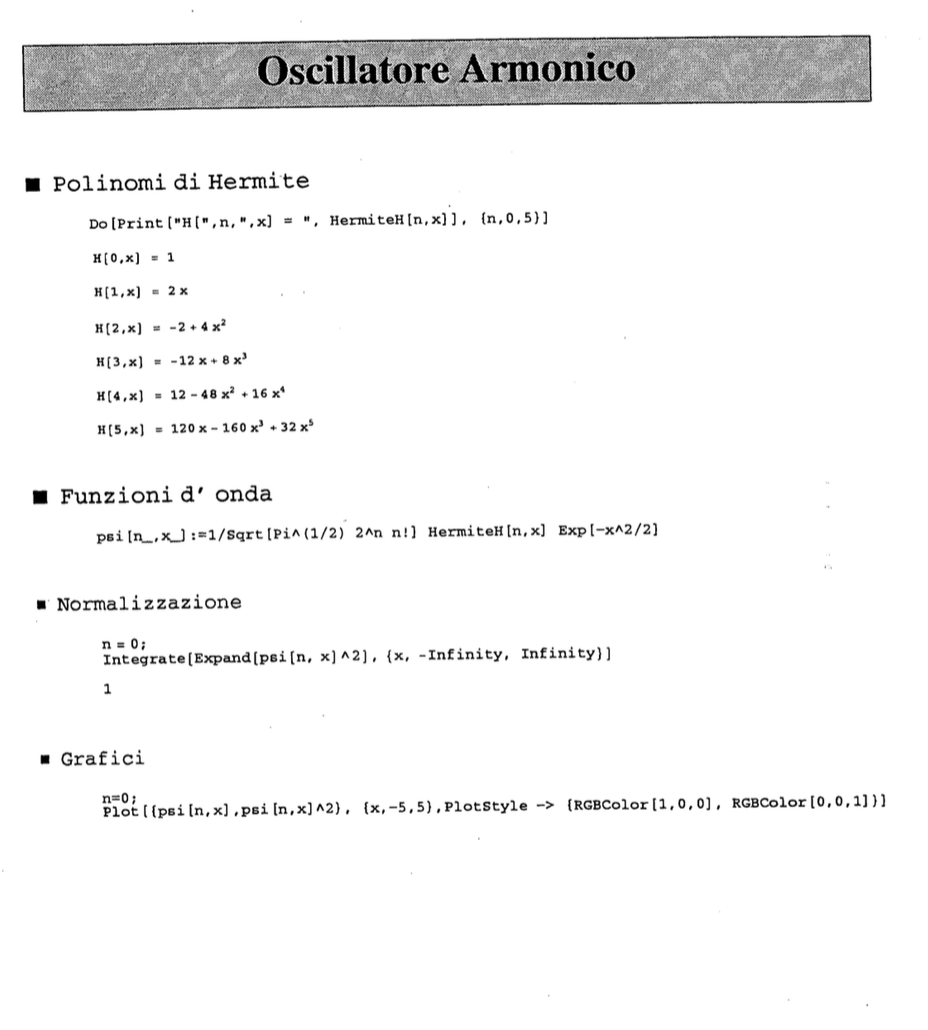
\includegraphics[width=\textwidth]{immagini/cap_11/polHer1.png}
\end{center}
\end{figure}

\begin{figure}[htbp]
\begin{center}
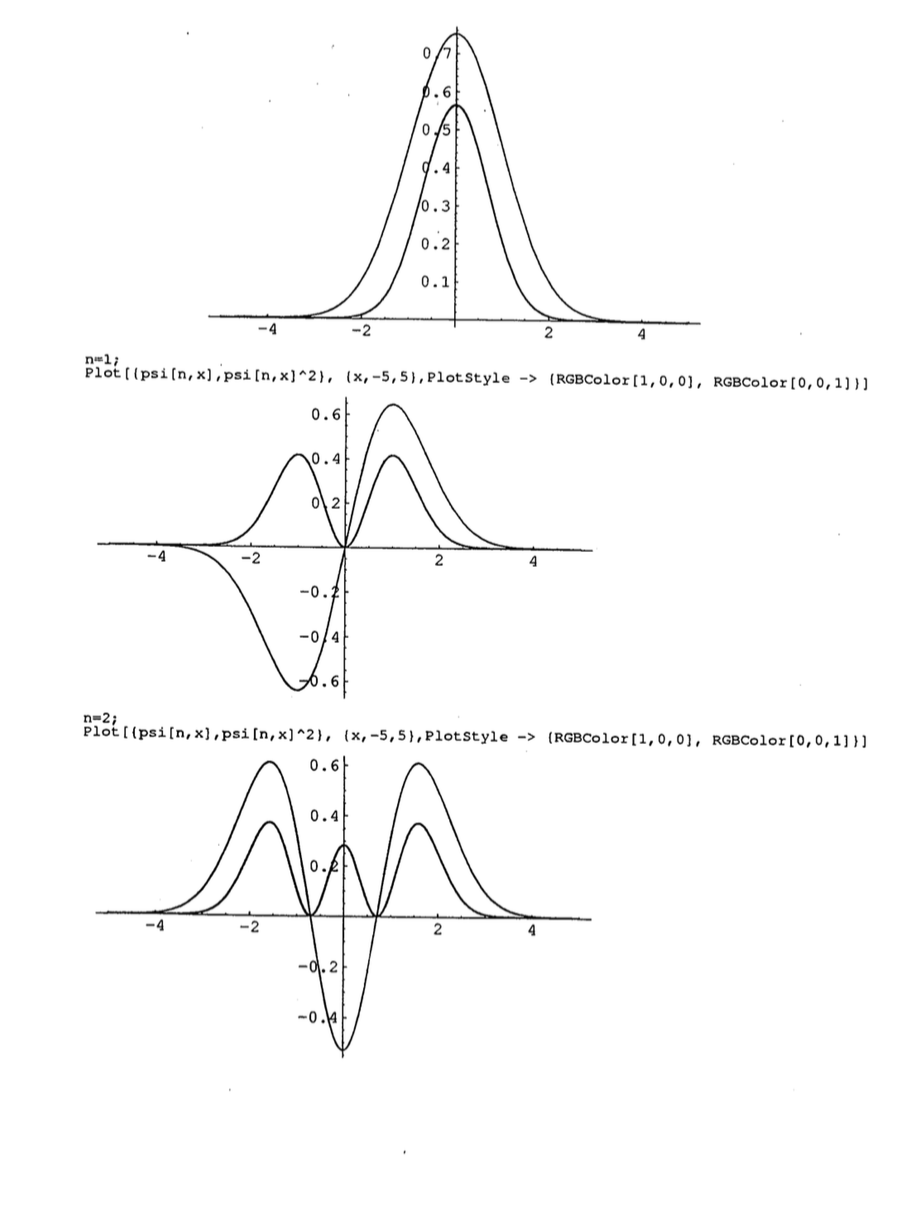
\includegraphics[width=\textwidth]{immagini/cap_11/polHer2.png}
\end{center}
\end{figure}
\end{document}
